% ****** Start of file aipsamp.tex ******
%
%   This file is part of the AIP files in the AIP distribution for REVTeX 4.
%   Version 4.1 of REVTeX, October 2009
%
%   Copyright (c) 2009 American Institute of Physics.
%
%   See the AIP README file for restrictions and more information.
%
% TeX'ing this file requires that you have AMS-LaTeX 2.0 installed
% as well as the rest of the prerequisites for REVTeX 4.1
% 
% It also requires running BibTeX. The commands are as follows:
%
%  1)  latex  aipsamp
%  2)  bibtex aipsamp
%  3)  latex  aipsamp
%  4)  latex  aipsamp
%
% Use this file as a source of example code for your aip document.
% Use the file aiptemplate.tex as a template for your document.
\documentclass[%
 aip,
% jmp,
% bmf,
% sd,
% rsi,
 amsmath,amssymb,
%preprint,%
 reprint,%
%author-year,%
%author-numerical,%
% Conference Proceedings
]{revtex4-1}

\usepackage{graphicx}% Include figure files
%\usepackage{dcolumn}% Align table columns on decimal point
\usepackage{fixme}
%\usepackage[mathlines]{lineno}% Enable numbering of text and display math
%\linenumbers\relax % Commence numbering lines
\usepackage[utf8]{inputenc}
\usepackage[T1]{fontenc}
\usepackage{mathptmx}
\usepackage{lipsum}
\usepackage{amsmath}
\usepackage{physics}
\usepackage{xparse}
\usepackage{bbm}
\usepackage{hyperref}
%\usepackage{multirow}
%\usepackage{makecell}
\graphicspath{{Pictures/}}

\renewcommand*{\figureautorefname}{Fig.}

\newcommand{\mytitile}{Effects of strong interaction between light and matter in a superconducting artificial molecule}
\begin{document}
	\preprint{AIP/123-QED}
	
	\title[\mytitile]{\mytitile\\~}
	
	\author{G.P. Fedorov}
	\email{gleb.fedorov@phystech.edu}
	
	\affiliation{ 
		Russian Quantum Center, Skolkovo village, Russia
	}%
	\affiliation{ 
		Moscow Institute of Physics and Technology, Dolgoprundiy, Russia
	}%
	
	\author{V.B. Yursa}
	\affiliation{ 
		Moscow Institute of Physics and Technology, Dolgoprundiy, Russia
	}%
	
	\author{A. Efimov}
	
	\affiliation{ 
		Moscow Institute of Physics and Technology, Dolgoprundiy, Russia
	}%

	\author{K. Shiyanov}

	\affiliation{ 
		Moscow Institute of Physics and Technology, Dolgoprundiy, Russia
	}%

	\author{A. Yu. Dmitriev}
	\affiliation{ 
	Moscow Institute of Physics and Technology, Dolgoprundiy, Russia
	}%

	\author{O.V. Astafiev}
	\affiliation{ 
		Moscow Institute of Physics and Technology, Dolgoprundiy, Russia 
	}%
	
	
	\date{\today}% It is always \today, today,
	%  but any date may be explicitly specified
	
	
	\begin{abstract}
		To build a full-scale quantum processor it is necessary to automate as many steps as possible on the physical, hardware level. Circuit quantum electrodynamics (cQED) is a contemporary architecture for dispersive readout and Purcell protection of superconducting qubits of various types, and thus it is necessary to develop software that is able to perform every kind of automatic calibration of such systems from scratch without any human participation. An important step towards this goal is to build a noise-insensitive and accurate computer vision tool to process three-dimensional spectroscopic data. In this work, we present and describe two scalable algorithms that are able to extract the Hamiltonian parameters of the cQED systems from spectroscopic data. 
	\end{abstract}
	
	\maketitle
\section{Introduction}
Over the past twenty years, superconducting artificial atoms (SAA) were used in numerous experiments confidently demonstrating the validity of fundamental quantum mechanical laws\cite{you2011atomic}. Due to synthetic nature of SAA, their Hamiltonians can be pre-designed and engineered, and this makes them a particularly versatile tool for studies in quantum optics. Notably, their parameters may be varied in such a wide range that novel physical effects previously inaccessible for natural systems may be directly observed. For example, the strong coupling regime when the coupling strength between light and a quantum system approaches 1\% of their frequency has been a major milestone for atoms, molecules, etc and was only reached using high-finesse cavities. In contrast, superconducting quantum systems have rapidly attained this landmark using \textit{circuit QED}\cite{wallraff2004strong} just in a few years after their first discovery\cite{chiorescu2004coherent} and have already surpassed other strongly-coupled systems in terms of coherence\cite{forn2019ultrastrong}. 
Moreover, SAA do not even require confined radiation to implement strong coupling with light: they may be coupled unprecedently strong with the free-propagating EM-waves in the on-chip 1D waveguides\cite{astafiev2010resonance} without having to use cavities at all. The Rabi frequency in this case may reach 50\% of the transition frequency\cite{deng2015observation} which is already the ultra-strong coupling regime.

In general, a quantum system exposed to strong external driving can experience various quantum phenomena explained by resonant single- and multi-photon transitions between energy levels. The most known examples are coherent population trapping, electromagnetically induced transparency (EIT)\cite{boller1991observation}, stimulated Raman adiabatic passage\cite{bergmann1998coherent} and Autler-Townes (A-T) splitting\cite{autler1955stark}. 

In this work, we are studying effects of light-matter interaction that occur in a system of two coupled artificial atoms: a superconducting artificial molecule (SAM). In our experiment, we use two transmons\cite{koch2007charge} interacting with each other through a cavity bus\cite{majer2007coupling}. Microwave radiation is applied to this system through a coplanar on-chip antenna and transmon states may be monitored by dispersive readout using the same coupling cavity \cite{chow2010detecting}.

It turns out that due to the strong interaction of SAM with the microwave drive, multiphoton transitions and the Autler-Townes effect are playing the crucial role in the phenomena that we have discovered. The A-T splitting has been observed before in atomic\cite{picque1976direct}, molecular systems\cite{tamarat1995pump}, quantum dots\cite{xu2007coherent}, and for SAA as well\cite{baur2009measurement, sillanpaa2009autler, novikov2013autler, suri2013observation, peng2018vacuum}. However, the previous studies have  only involved just a single SAA and have demonstrated only the standard spectral signatures known from the quantum optics (see Appendix \ref{sec:3-level-at}); instead, a diatomic SAM allows to observe some qualitatively new spectral manifestations of the effect. Remarkably, besides its fundamental value, this experiment may be useful for future quantum computers: a quantum engineer should consider the observed behaviours as unwanted, and thus careful control of the driving power must be employed to avoid them (for instance, as we will show, the bSWAP gate\cite{poletto2012entanglement} is directly affected).

The manuscript consists of four main parts and an Appendix. Section I is this introduction; Section II is devoted to the approaches that were used in our study; Section III contains the results of our experimental and theoretical research; finally, in Section IV we make a conclusion of our work and discuss future prospects. The Appendix contains important details of the theoretical framework that we use to model the observed processes.

\section{Methods}

In this section, we provide the mathematical formulation of the employed models, specify the numerical approaches that were used in simulations and describe the experimental equipment and some measurement aspects.  

\subsection{Experiment}

\subsubsection{Device design and fabrication}
We have designed the SAM as a pair of transmon (Xmon\cite{barends2013coherent}) SAAs with asymmetric SQUIDs\cite{hutchings2017tunable} coupled to a single notch-type\cite{probst2015efficient} $\lambda/4$ resonator which serves both to couple\cite{majer2007coupling} the qubits and for the joint\cite{chow2010detecting} readout of their states. In \autoref{fig:experiment}~(a) the optical photograph of the device is shown depicting the layout of the components. The resonator in its upper part is connected to a coplanar waveguide through which the readout is performed. In its lower part, it is coupled to the transmons by a dual ``claw''\cite{barends2013coherent} coupler. Flux lines that allow independent control of the $ge$ transitions of the transmons are coming from the sides. Finally, the excitation waveguide coming from below directs microwave signal towards the SAM. In \autoref{fig:experiment}~(b) the equivalent electrical circuit of the device. The resonator fundamental mode is approximated as an LC-circuit (in the middle), the transmons are shown in colour on the sides as the LC-circuits as well, but with tunable non-linear inductances. The capacitively coupled excitation line is also shown in green. Finally, in \autoref{fig:experiment}~(c) we show schematically the $ge$ transitions of the transmons depending on the external magnetic flux. Since the effective junction of the first transmon is larger, its spectrum (orange) lies higher in frequency the spectrum of the second qubit (blue). Using both coils, it is possible to align them so that the lower sweet-spot of the orange qubit. As will be shown, this arrangement allows to see multiple energy level intersections including higher transmon levels, and thus we are measuring the SAM in the region shown with the dashed rectangle.



\begin{figure}
	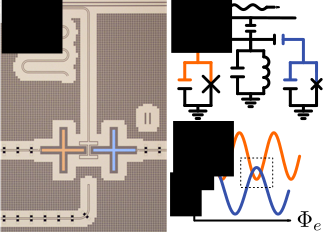
\includegraphics[width=\linewidth]{experiment}
	\caption{Experimental device. \textbf{(a)} Optical photograph of the device (false coloured). Two transmons (orange, 1 and blue, 2) are coupled capacitively to a $\lambda/4$ coplanar resonator. From both sides come the frequency control flux lines, and from below a microwave excitation waveguide is connected (green). \textbf{(b)} The equivalent electrical circuit. Tunable Josephson junctions are in fact SQUIDs with magnetic flux control. \textbf{(c)} Frequencies of the $ge$ transitions of the transmons $\omega_1(\Phi_e)$ and $\omega_2(\Phi_e)$ depending on the external magnetic flux (coloured correspondingly). In this work, we concentrate on the area inside the dashed rectangle.}
	\label{fig:experiment}
\end{figure}


\begin{table}
	\begin{tabular}{c|c|c|c}
	Parameter & Resonator & Qubit 1 & Qubit 2\\\hline
	$\omega/2\pi$ [GHz] & 7 & 5.12 - 6.9 & 4 - 5.45\\
	$\Gamma_1$ [$\mu$s] & 0.1 & $\leq$ 10  &  $\leq$ 5\\
	$\Gamma_2$ [$\mu$s] & - & $\leq$ 7  &  $\leq$ 1
	\end{tabular}
	\caption{Device parameters}
\end{table}


\subsubsection{Experimental parameters}
\subsubsection{Experimental setup}
The sample was measured in laboratory of artificial quantum systems at Moscow Institute of Physics and Technology. Cryogenic equipment was
represented by BlueFors LD250 dilution refrigerator, with base temperature of 16 mK. The microwave equipment included KEYSIGHT PNA-L N5232A 300 kHz-20 GHz vector network analyser, Agilent MXG N5183B 9 kHz - 40 GHz analog signal generator. The sample was 
flux biased using YOKOGAWA GS200 current source.

Microwave line was thermalized with 60 dB of attenuation, additional 20 dB of attenuation were introduced on a directional coupler which added the second tone from the $\mu$-wave source. After leaving the sample the signal passed through two isolators and a hybrid coupler. Finally, the signal was amplified with 4-8 GHz LNF amplifier at 4 K and a with a room-temperature amplifier.



\subsection{Theoretical description of the system}

A single transmon SAA can be considered as an oscillator with a quartic perturbation describing the leading-order anharmonicity. Therefore, in the main text we avoid using the standard charge and phase operators (this approach is covered Appendix) and write down its Hamiltonian using the annihilation operator $\hat b$:
\begin{equation}
\hat H_{tr}/\hbar = \omega \hat b^{\dagger}\hat b +\frac{1}{2}\alpha \hat b^{\dagger}\hat b(\hat b^{\dagger}\hat b-1),
\end{equation}
where $\omega$ is its $\ket{0}\rightarrow\ket{1}$ (or the  $ge$) transition frequency and $\alpha$ is the anharmonicity of the transmon. Additionally, by applying external magnetic flux $\Phi_e$ it is possible to control $\omega = \omega(\Phi_e)$\cite{koch2007charge}.


To induce state transitions in a transmon one should irradiate it by a monochromatic external microwave signal of frequency $\omega_d$ using a capacitively coupled transmission line. The interaction term between the transmon and this classical EM field is then modelled by the following operator: 
\begin{equation}
\hat H_{dr}/\hbar = \Omega\cos(\omega_d t)(\hat b+\hat b^{\dagger}),
\end{equation}
where $\Omega$ stands for the frequency of the Rabi oscillations between $\ket{0}$ and $\ket{1}$.

Now, for the molecule composed of two coupled transmons, the complete Hamiltonian contains two terms describing each of them in isolation (with the corresponding annihilation operators $\hat b$ and $\hat c$ and the $ge$ frequencies $\omega_{1,2}$), two terms representing the interaction of each transmon with the driving field at the same frequency $\omega_d$, and the qubit-qubit interaction term:
\begin{equation}\label{Hsystem}
\hat H = \hat H_{tr1}+\hat H_{tr2}+\hat H_{dr1}+\hat H_{dr2}+\hat H_{int},
\end{equation}
where $\hat H_{int}/\hbar= J (\hat b +\hat b^\dag)(\hat c+\hat c^{\dagger})$ is the transverse interaction between the atoms.

Besides the unitary evolution, we take into account the incoherent processes of relaxation and dephasing for each transmon. They are modelled using the Lindblad equation with the following collapse operators:
\begin{equation}\
\begin{split}
\hat{\mathcal{O}}_{\gamma, 1} = \sqrt{\gamma_1}\, \hat b,\ 
\hat{\mathcal{O}}_{\phi, 1} = \sqrt{2\gamma_{\phi,1}}\, \hat b^\dag \hat b,\\
\hat{\mathcal{O}}_{\gamma,2} = \sqrt{\gamma_2}\, \hat c,\ 
\hat{\mathcal{O}}_{\phi,2} = \sqrt{2\gamma_{ \phi,2}}\, \hat c^\dag \hat c.
\end{split}
\end{equation}
As one can see, the collapse operators are in a separable form, i.e. acting only upon a single transmon each. This is a valid approach until the coupling strength $J$ is not too large\cite{beaudoin2011dissipation}. Therefore, the complete evolution equation for the system density matrix $\hat \rho$ is
\begin{equation}
\partial_t \hat \rho = \frac{i}{\hbar} [\hat \rho, \hat H] + \sum_{\alpha, i} \mathcal{D}[\hat{\mathcal{O}}_{\alpha, i}] \hat \rho, \label{eq:master}
\end{equation}
where $\mathcal{D}[\hat{\mathcal{O}}]\hat \rho = \hat{\mathcal{O}} \hat \rho \hat{\mathcal{O}}^\dag - \frac{1}{2}\{ \hat{\mathcal{O}}^\dag \hat{\mathcal{O}}, \hat \rho\}$.



\subsection{Master equation solution in \textit{qutip}}

Numerical simulations are crucial in studying the equation \eqref{eq:master} since is does not allow an analytical solution. We have been using the \textit{qutip}\cite{johansson2013qutip} quantum optics toolbox to simulate the dynamics and find the steady state of the system for various parameter combinations of the Hamiltonian.

Two distinct modes of operation were used during the 


\section{Results}

\subsection{\label{sec:level1} Experimental and numerical parts}
Two tone spectroscopy was found experimentally and shows good agreement with modelling data \autoref{fig:two-tone}. 

\begin{figure*}
	\centering
	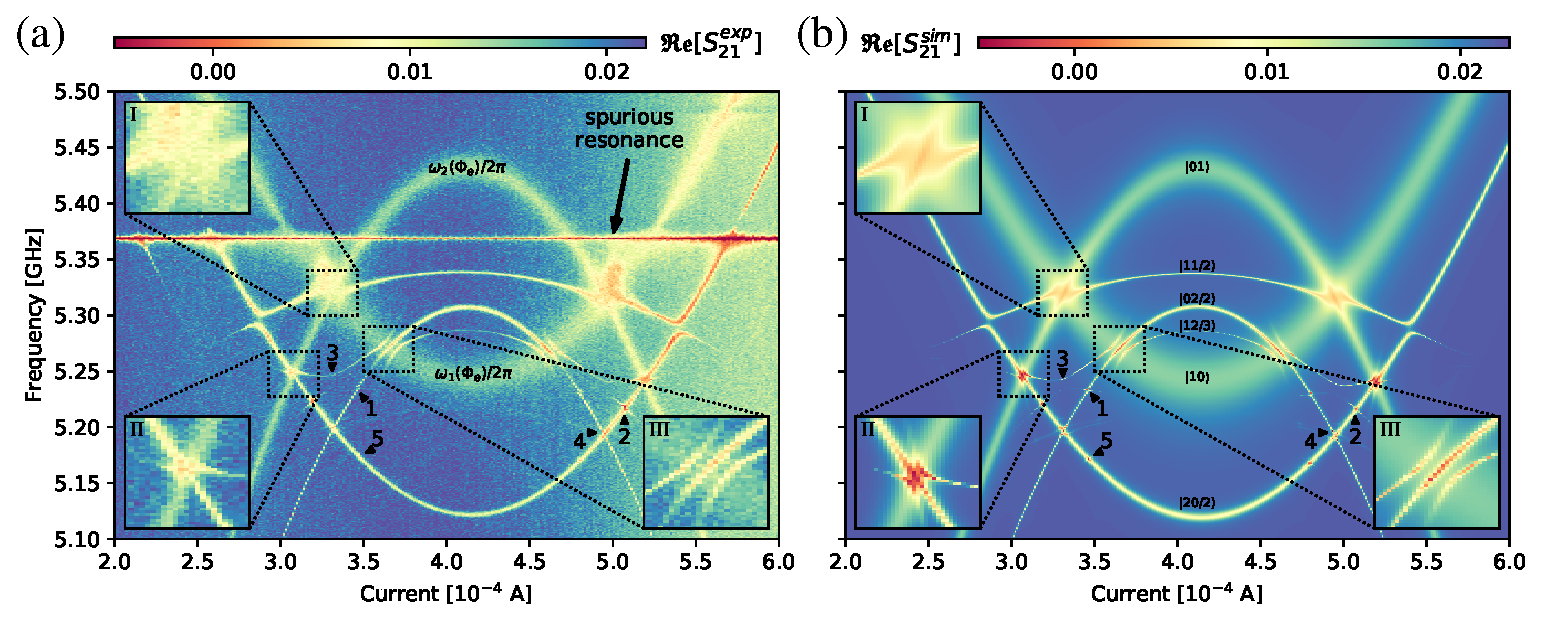
\includegraphics[width=\linewidth]{main_picture}
	\caption{Two-tone spectroscopy: \textbf{(a)} Experiment;\textbf{(b)} Modelling ; the colorbar is common.  Clear flux-dependent transmon transitions are visible.}
	\label{fig:two-tone}
\end{figure*}

\begin{figure*}
	\centering
	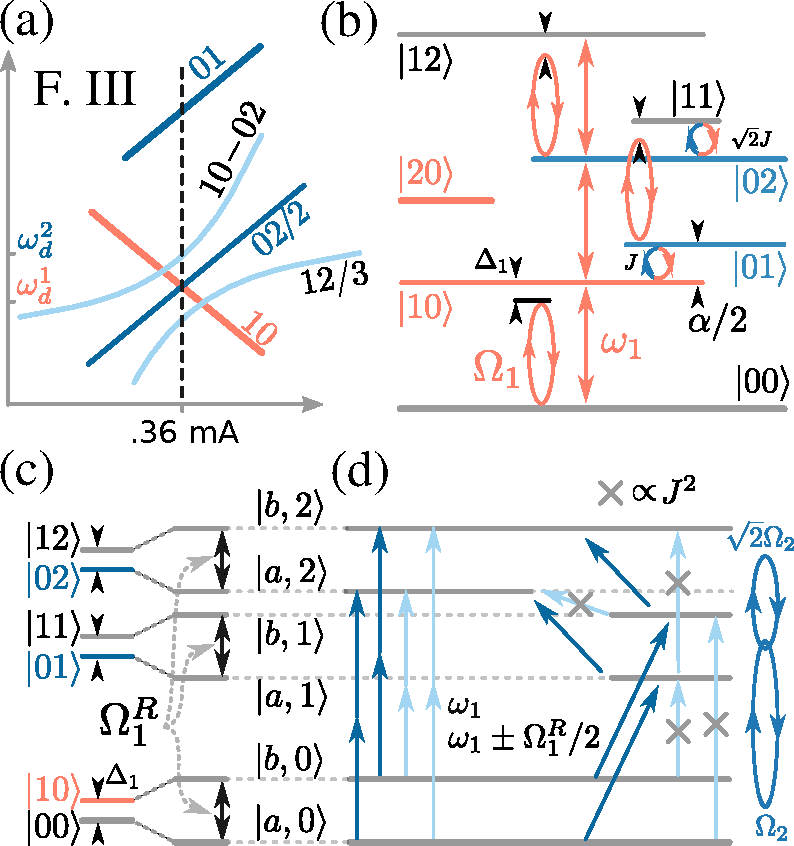
\includegraphics[width=.9\linewidth]{main_scheme}
	\caption{Explaining the origin of the AT satellites. \textbf{(a)} System level structure at 3.65 mA. At this current, the first transmon (orange) is below the second one (blue) exactly by $\alpha/2$ ($\omega_2 - \omega_1 = \alpha/2$), and thus $E_{02} - E_{10} = \hbar\omega_1$. Since $E_{12} - E_{02} = \omega_1$ as well, both $00\rightarrow 10$, two-photon $00 \rightarrow 02/2$ and three-photon $00\rightarrow 12/3$ transitions can occur around the same frequency of $\omega_1$. During the two-tone spectroscopy, the first transmon is driven by a strong signal of amplitude $\Omega_1$ (possibly, at a small detuning $\Delta_1$ from $\omega_1$ shown in green). The transmon-transmon interaction in RWA conserves the number of excitations and is depicted as orange-blue circles. \textbf{(b)} Moving to the frame rotating with the drive of the first transmon, we make all the states $\ket{0j},\ket{1j}$ nearly degenerate (in fact, now the first transmon splitting equals $\Delta_1$). However, the presence of a strong excitation lifts the degeneracy and the splitting changes to $\Omega_1^R = \sqrt{\Omega_1^2 + \Delta_1^2}$ (the first transmon becomes light-dressed). \textbf{(c)} Transitions in the light-dressed system when the second qubit is excited (level subspaces coupled by the corresponding drive operator are shown as blue ellipses). In the left part of the panel, all possible two-photon transitions near $\omega_1$ are depicted. The structure of the levels gives rise to three cases: the green transitions are not shifted in frequency, the orange are red-shifted by $\Omega_R^1/2$ and the blue are blue-shifted by $\Omega_R^2/2$. However, as shown in the right part of the panel, without the transmon-transmon interaction the satellite transitions are forbidden due the selection rule: $\bra{a,j}\hat{\mathbbm{1}}\otimes \hat n_2 \ket{b, j+1} = 0$ since $\braket{a}{b} = 0$. When the coupling equals $J$, the dispersive approximation yields $\bra{a,j}\hat{\mathbbm{1}}\otimes \hat n_2\ket{b, j+1}\propto J^2/(\omega_1-\omega_2)^2$ and the satellites become visible. Remarkably, due to the two-photon nature of the transitions, the Autler-Townes splitting in this case will be two $\Omega_1^R$.}
	\label{fig:main_scheme}
\end{figure*}

We obtain illustrative example of dressed states\autoref{fig:difdrive}. On this figure the microwave drive acts only on the one of qubits. 
\begin{figure}
	\centering
	\includegraphics[width=\linewidth]{drawing}
	\caption{Drive acts on the one of qubit, with different amplitude 100,200,300 MHz}
	\label{fig:difdrive}
\end{figure}


\subsection{Theoretical description of the observed spectral lines}
For the three-level system, the A-T effect is described in Appendix \ref{sec:3-level-at}. Let's consider our system (\autoref{Hsystem}) in rotating frame. Moving to this frame is achieved by the rotation:
\begin{equation}
R = \exp(-i\omega_d t (b^{\dagger}b+c^{\dagger}c))
\end{equation}  
After this transformation the effective Hamiltonian can be found from equation:
\begin{equation}
H_{system}^R = R^{\dagger}H_{system}R-iR^{\dagger}\dot{R}
\end{equation}

From the simulation follows that a two-level approximation for first qubit and three-level approximation for second is sufficient to observe the effect we are interested in. The Hamiltonian in matrix form is given by the following expression:
\begin{widetext}
	\begin{equation}\label{matrix} 
	\text{$H^R$} = \left(\begin{matrix}
	0 & \text{$\Omega_1/2 $} & \text{$\Omega _2$} e^{i \text{$\delta_{\omega}$} t}/2 & 0 & 0 & 0 \\
	\text{$\Omega_1/2 $} & \text{$-\Delta_1 $} & J & \text{$\Omega_2$} e^{i \text{$\delta_{\omega}$} t}/2 & 0 & 0 \\
	\text{$\Omega_2$} e^{-i \text{$\delta_{\omega} $} t}/2 & J & -\text{$\Delta_2 $} &
	\text{$\Omega_1$/2} & \sqrt{2} \text{$\Omega_2$} e^{i \text{$\delta_{\omega}$} t}/2 & 0 \\
	0 & \text{$\Omega_2$} e^{-i \text{$\delta_{\omega} $} t}/2 & \text{$\Omega_1/2$} &
	\text{$-\Delta_2 -\Delta_1$} & \sqrt{2} J & \sqrt{2} \text{$\Omega_2$} e^{i \text{$\delta_{\omega}
			$} t}/2 \\
	0 & 0 & \sqrt{2} \text{$\Omega_2$} e^{-i \text{$\delta_{\omega}$} t}/2 & \sqrt{2} J &
	\text{$\alpha$}-2 \text{$\Delta_2$} & \text{$\Omega_1/2$} \\
	0 & 0 & 0 & \sqrt{2} \text{$\Omega_2$} e^{-i \text{$\delta_{\omega} $} t}/2 & \text{$\Omega_1/2
		$} & \text{$\alpha$}-2 \text{$\Delta_2$}- \text{$\Delta_1$} \\
	\end{matrix}\right)
	\end{equation}
\end{widetext}
Where $\Omega_1$, $\Omega_2$ - amplitudes of the drives, $\Delta_1 = \omega_d-\omega_{tr1}=0$,$\Delta_2 = \omega_d-\omega_{tr2}$.
Let's consider the Hamiltonian (\autoref{matrix}) in details. Divide it into three parts: time-dependent $(V_t)$, the part responsible for the interaction between the qubits $(V_J)$ and all the rest $(H_0)$.
\begin{equation}
	H^R=H_0+V_J+V_t
\end{equation}
The $\Omega_1\gg \Omega_2,\Delta_2\gg J$, so the driven field on the first qubit is strong and form the dressed states defined by the Hamiltonian $H_0$.
The Hamiltonian $H_0$ is station and we can find eigenvectors and eigenvalues. The drive on the second qubit is weak with very low intensity, so we can neglect any perturbation introduced by second drive on the position, width os the dressed states.
Firstly, we consider the system of non-interacting qubits $(J=0)$. In this case some transitions are prohibited and the splitting we are interested in is not observed. 
Therefore a non-zero interaction between qubits is necessary to observe AT effect.

After that according to the perturbation theory (with perturbation $V_J$) to $H_0$ we found the first-order corrections to the wave functions. We can use Fermi Golden Rule to find the probability of transition.
\appendix

\section{Standard Autler-Townes effect for a three-level atom} \label{sec:3-level-at}

The underlying cause of the A-T effect is the dressing of the atomic levels by strong EM radiation. There are two equivalent mathematical models for it: the light may be classical or quantized.

\begin{figure}
	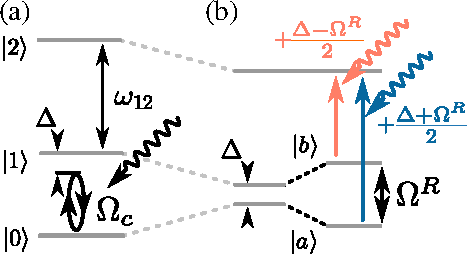
\includegraphics[width=\linewidth]{intro_scheme}
	\caption{Illustrating the A-T splitting by  the classical driving in the rotating frame ($\hbar=1$ here). \textbf{(a)} The three-level system is driven strongly by a ``coupler'' tone of amplitude $\Omega$ at frequency $\omega_{01}-\Delta$. It induces Rabi oscillations between $\ket{0}$ and $\ket{1}$ at the generalized Rabi frequency $\Omega_R = \sqrt{\Omega^2 + \Delta^2}$. \textbf{(b)} Moving to the frame rotating with the drive, we effectively change the $\ket{0}\rightarrow \ket{1}$ transition frequency to $\Delta$. However, when RWA is applied and Hamiltonian is re-diagonalized, the splitting between two lowest levels (dressed states $\ket{a}$ and $\ket{b}$) becomes $\Omega^R$. Now, the experimenter may observe a doublet transition from these levels to the state $\ket{2}$ at frequencies $\omega_{12}+(\Delta \pm \Omega^R)/2$.} 
	\label{fig:at-standard}
\end{figure}

\paragraph{Classical derivation.} In the classical case, the mathematical description goes as follows. At first, there is a three-level system which is driven by a strong radiation with an amplitude $\Omega_1$ at a frequency detuned by $\Delta$ from the $\ket{0}\rightarrow \ket{1}$ transition with a frequency $\omega_{01}$. Additionally, we have a weak probe radiation at a frequency $\omega_{p}$ and with an amplitude $\Omega_2$ between $\ket{1}$ and $\ket{2}$. This step is illustrated in \autoref{fig:at-standard}~(a). The Hamiltonian for such system is as follows:

\begin{equation*}
\hat H^c_0 = \left[\begin{matrix}
0 & \Omega_{1} \cos{\left(\omega_{01}- \Delta \right)t} & 0\\
\Omega_{1} \cos{\left(\omega_{01} - \Delta \right)t}   & \omega_{01} &\Omega_{2} \cos\omega_p t  \\
0 & \Omega_{2} \cos{\omega_p t}  & \omega_{02}\end{matrix}\right].
\end{equation*}

Next, we move to the rotating frame by using an operator
\[
\hat R = \left[\begin{matrix} 
1 & 0 & 0\\0 & e^{i t \left(\omega_{01}- \Delta\right)} & 0\\0 & 0 & e^{i t \left(\omega_{01}- \Delta\right)}\end{matrix}\right].
\]
Note here that level $\ket{2}$ is also rotated: this is convenient to preserve the frequency of the driving term with $\Omega_2$. The new Hamiltonian should be calculated as follows: $\hat H_1 = \hat R^\dag \hat H_0 \hat R + i \dot{\hat{R}}^\dag \hat R$. The level structure without driving  is shown in the left part of \autoref{fig:at-standard}~(b). Applying the RWA, we obtain:
\begin{equation*}
\hat H^c_1 = \left[\begin{matrix}0 &\Omega_{1}/2 & 0\\\Omega_{1}/2 & \Delta & \Omega_{2} e^{i t \omega_p}/2\\0 & \Omega_{2} e^{-i t \omega_p}/2 & \omega_{02} - \omega_{01}+\Delta \end{matrix}\right].
\end{equation*}

Next, moving to the basis where the upper left 2x2 corner is diagonal (the right part of \autoref{fig:at-standard}~(b)), we obtain:

\begin{equation*}
\hat H^c_3 = \left[\begin{matrix} 
\frac{\Delta}{2} - \frac{\sqrt{\Delta^{2} + \Omega_{1}^{2}}}{2} & 
0 &
\frac{\Omega_{2} e^{i t \omega_{p}}}{2}\sin(\theta)
\\
0 & 
\frac{\Delta}{2} + \frac{\sqrt{\Delta^{2} + \Omega_{1}^{2}}}{2} & 
\frac{\Omega_{2} e^ {i t \omega_p}}{2}\cos(\theta)
\\
\frac{\Omega_{2} e^{-i t \omega_{p}} }{2}\sin(\theta) & 
\frac{\Omega_{2} e^{-i t \omega_{p}}}{2} \cos(\theta) & 
\omega_{12} +\Delta 
\end{matrix}\right].
\end{equation*}

One may see that now resonant conditions for the probe drive are $\omega_p = \omega_{12} + \dfrac{(\Delta \pm \Omega^R)}{2}$, where $\Omega^R = \sqrt{\Omega_1^2 + \Delta^2}$, $\omega_{12} = \omega_{02}- \omega_{01}$, and its amplitude is renormalized by an angle $\theta,\ \tan 2\theta = -\frac{\Omega_1}{\Delta}$.


\paragraph{Quantum derivation.} For the fully quantum interpretation, we model the incident radiation at the frequency $\omega_{01}-\Delta$ as a single-mode quantum oscillator which is coupled to the system. The Hamiltonian for this model will be as follows:
\[
\begin{split}
\hat H^q_0 = \omega_{01} \ket{1}\bra{1} + \omega_{02} \ket{2}\bra{2} + (\omega_{01}-\Delta) \hat a^\dag \hat a + \\\ g (\hat a^\dag + \hat a)\otimes (\ket{1}\bra{0}+\ket{0}\bra{1}),
\end{split}
\]
where $g$ is the coupling strength and $a$ is the photon annihilation operator. After moving to the rotating frame with $\hat R = \exp[i t (\omega_{01}-\Delta)(\hat a^\dag \hat a + \ket{1}\bra{1}+\ket{2}\bra{2})]$ and applying the RWA, the Hamiltonian transforms into
\[
\begin{split}
\hat H^q_1 = \Delta \ket{1}\bra{1} + (\omega_{12}+\Delta) \ket{2}\bra{2} + \\\ g \left[\hat a^\dag \otimes \ket{0}\bra{1} + \hat a \otimes \ket{1}\bra{0}\right].
\end{split}
\]
If we presume that the resonator is in a coherent state $\ket{\alpha e^{-it(\omega_{01}-\Delta)}}$ with $\langle N\rangle = \alpha^2$ photons and average $\hat H_1^q$ over the resonator subspace, we from the interaction term will obtain again the classical driving strength $\Omega_1 = 2 \sqrt{\langle N \rangle} g$ in correspondence with the classical driving case. Similarly, the energy levels $\ket{1, N-1}$ and $\ket{0, N}$ become mixed due to the coupling, and their splitting changes from $\Delta$ to $\Omega_R = \sqrt{\Omega_1+\Delta}$. The following steps completely reproduce the classical case if we add the probe tone $\Omega_2$ in the last equation.

\section{Theoretical description of two-photon process}





\section{Text}


In order to determine which transitions correspond to the lines, the stationary Schrödinger equation was solved \autoref{fig:spectr} in three-level approximation for both of qubits. With the Hamiltonian of the system:
\begin{equation}
	H_{system} = H_{tr1}\otimes\mathbbm{1}+\mathbbm{1}\otimes H_{tr2}+H_{int}
\end{equation}
\begin{figure}[h]
	\centering
	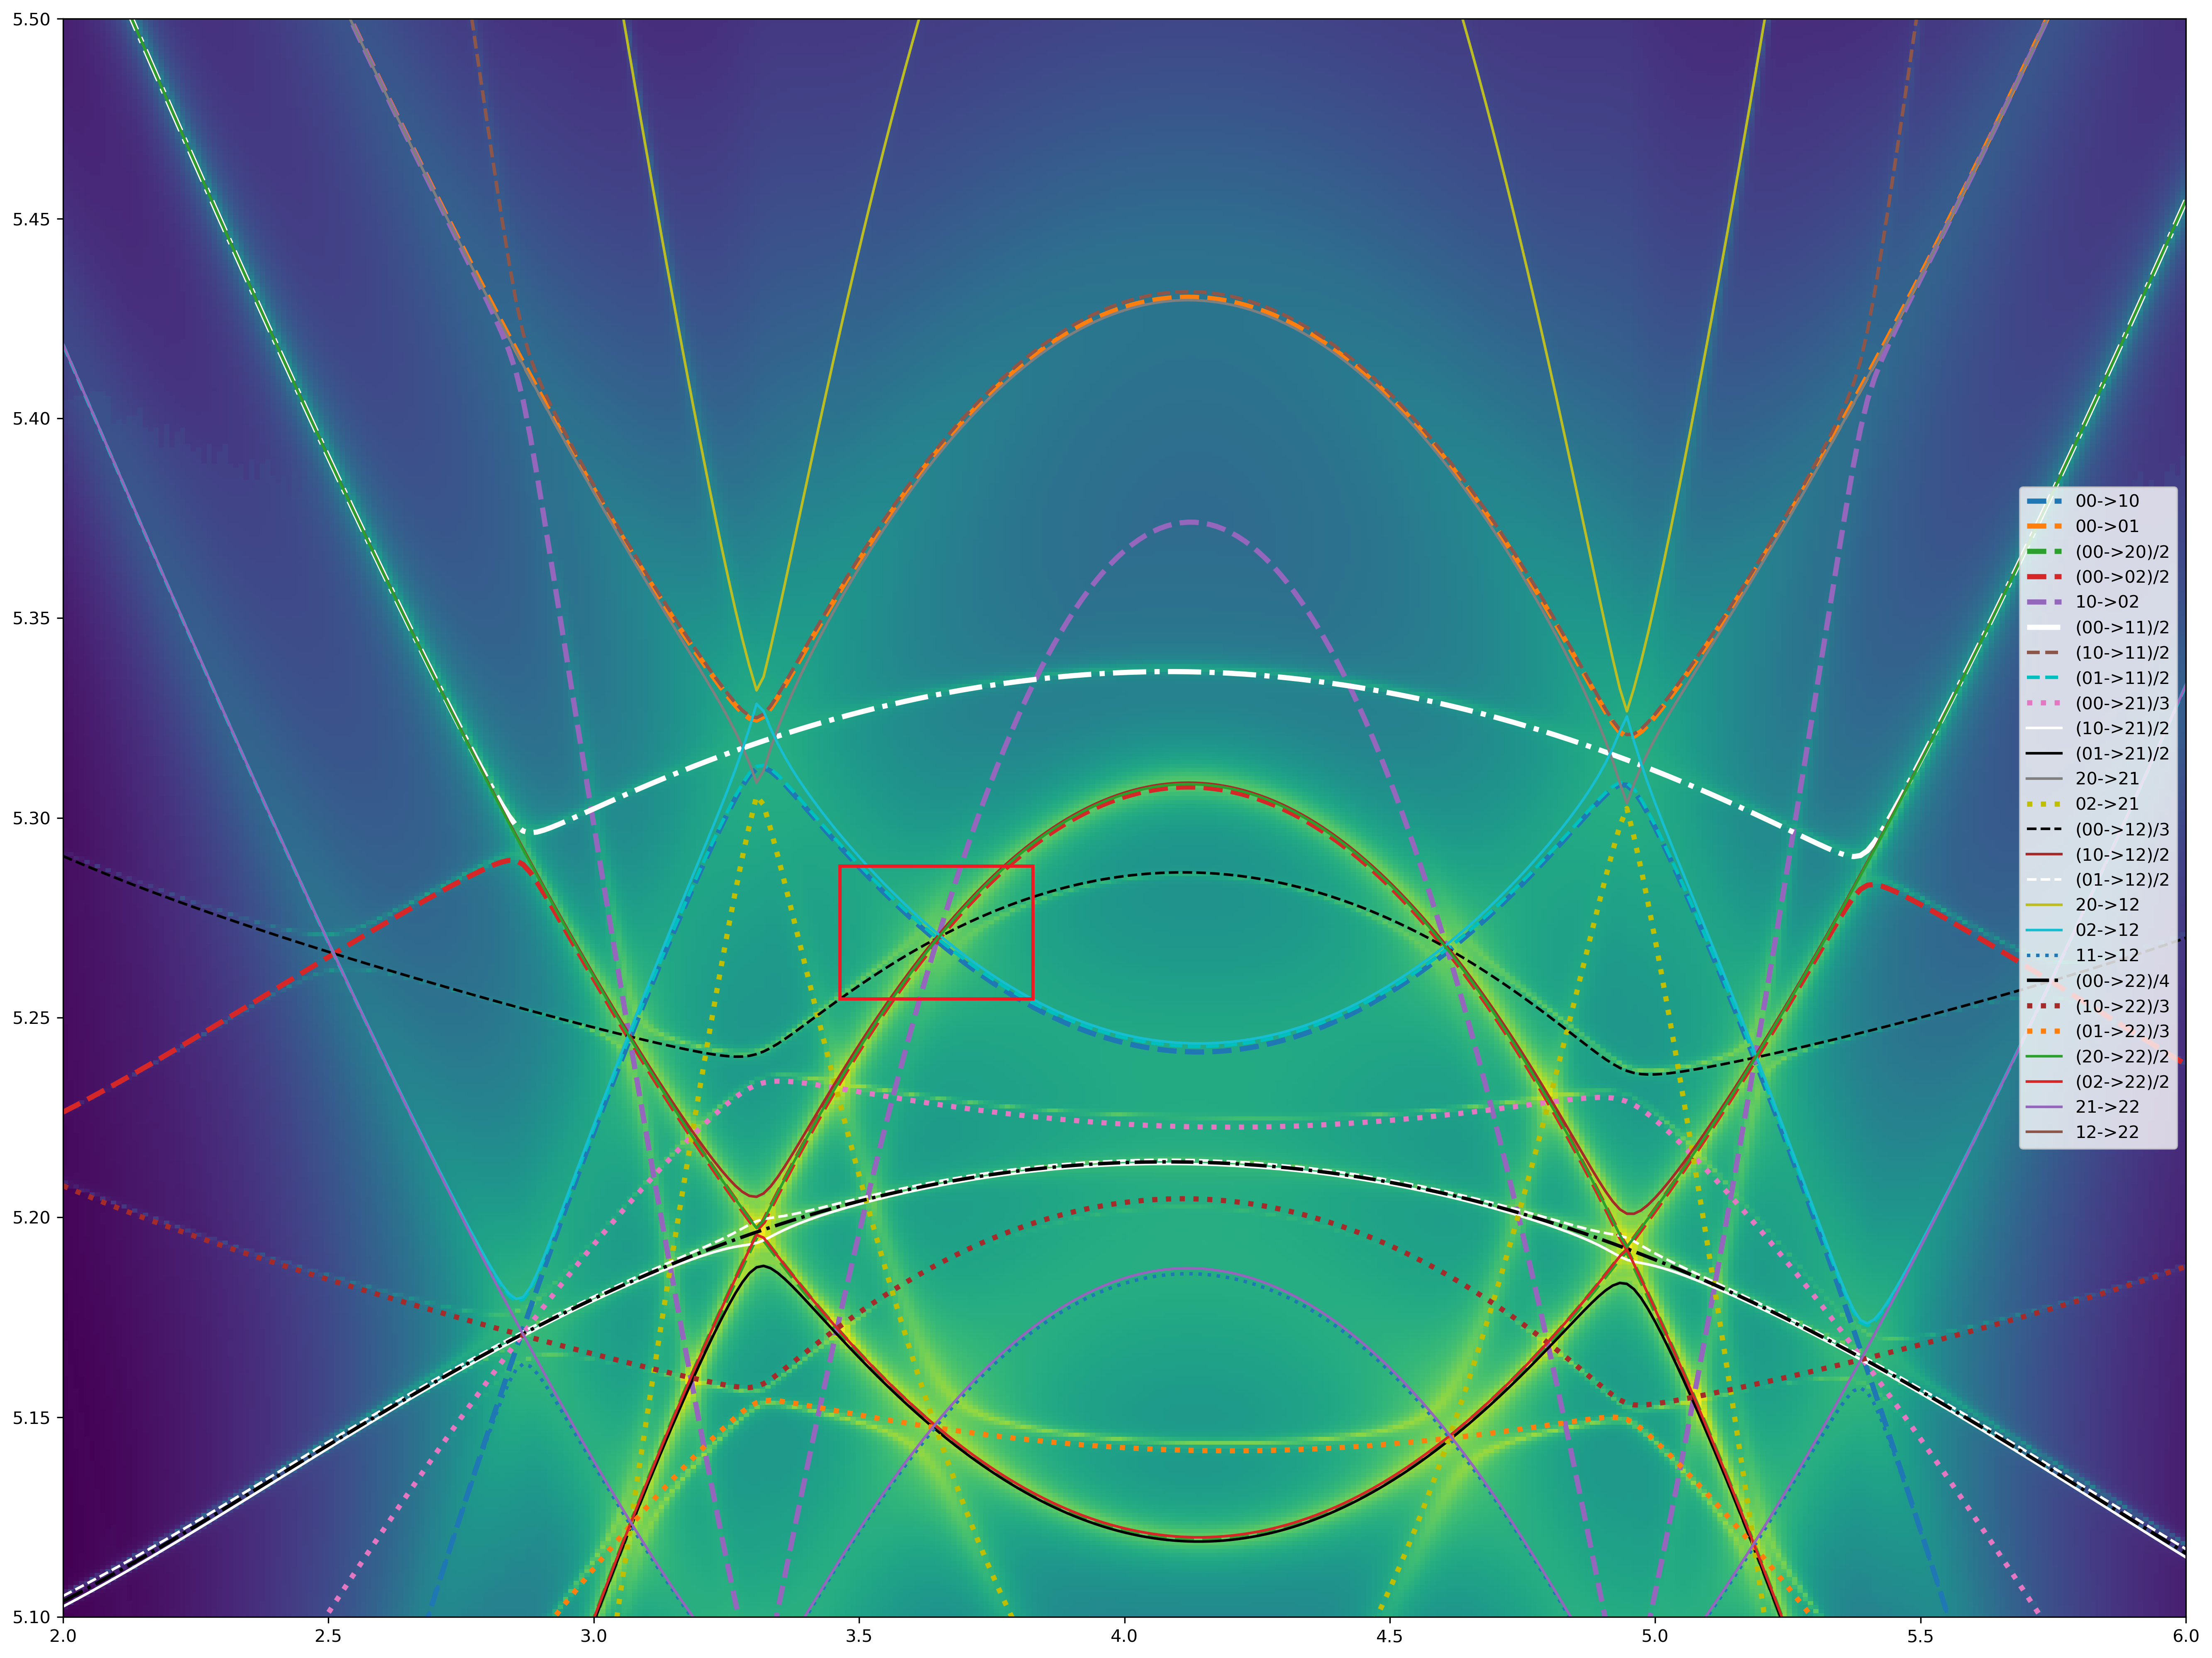
\includegraphics[width=\linewidth]{spectr}
	\caption{Two-tone spectroscopy with transitions lines. In the red frame, four transitions intersect, three of which originate from the state $\ket{00}$ to $\ket{10}$, two-photon
		$\ket{02}$, three-photon
		$\ket{12}$ and the fourth from  $\ket{10}$ to  $\ket{02}$, where $\ket{ij}$ denote the $ij-th$ energy eigenstate of the transmon system, i,j represent first and second qubit respectively}
	\label{fig:spectr}
\end{figure}


 Let's described the anti-crossing highlighted in red in the picture. 
 



\bibliography{papers_bibliography}% Produces the bibliography via BibTeX.	
\end{document}